\documentclass[12pt, letterpaper]{article}
\usepackage[margin=1in]{geometry}
\usepackage{graphicx}
\usepackage{amsmath}
\usepackage{amssymb}
\usepackage{tikz}
\graphicspath{ {figures_EC102/} }

\title{
	{EC102 Macroeconomics}\\
	{\large{Professor Franceso Caselli}}\\
	{\large{Revision Document}}
}
\author{Cedric Tan}
\date{April 2019}

\begin{document}
\maketitle
\abstract{

This is a review of macroeconomic lectures by Franceso Caselli in Lent Term of 2019. The notes are mine fully and may not be authentic to the lecturer's as they have been modified.

The format of this material is usually recounted slide by slide but some slides may be merged together as the material fits appropriately with one another.
}

\newpage
\tableofcontents
\newpage

\section{Introduction to Macro}
Macroeconomics is about the performance of the economy overall. Topics that will be covered in this course are as follows:
\begin{itemize}
	\item Long-run Economic Growth
	\item Booms and Recessions
	\item Inflation and Deflation
	\item Unemployment
	\item Financial, Currency and Sovereign Debt Crises
\end{itemize}

Further to that, here are some of the big macroeconomic issues that we are facing today in (\textbf{April 2019:})
\begin{itemize}
	\item Why are we growing so slowly and is the slowdown permanent?
	\item What are the consequences of \textbf{Brext} for UK growth?
	\item Has austerity been a good idea? In the UK? In the Eurozone?
	\item Why is inflation so low and what should Central Banks do about it?
	\item What will happen when Central Banks end \textbf{Quantitative Easing?}
	\item Will lower-income countries ever catch up to the high-income ones?
	\item Will there be a financial crisis in China?
	\item Have we done enough to prevent a new financial crisis?
\end{itemize}

\begin{center}
	\textbf{Colin O'Shea:} \textit{Market sentiment always dictates what will happen. Policy implementation may not always work as it is dependent on sentiment.}
\end{center}

\begin{center}
	\Large{\textbf{Welcome to macroeconomics}}
\end{center}

\newpage
\section{Economic Growth}
We will begin with a definition of Economic growth:

\textit{It is the \textbf{long run} changes in \textbf{material living standards.} \\}

Long run means:
\begin{itemize}
	\item Persistent changes over time
	\item One generation compared to the previous
	\item Definitely not a quarter by quarter analysis \\
\end{itemize}

Material means:
\begin{itemize}
	\item Food, housing: these are \textbf{physical objects}
	\item Education, healthcare
	\item Income to access these goods and services
\end{itemize}

\subsection{Preliminary Questions on Growth}
Further to this, we will ask some preliminary questions on growth to get the gears running:
\begin{itemize}
	\item How do we measure it?
	\item Is indefinite growth feasible? i.e. \textbf{Growth forever on an upwards trend?}
	\item Is indefinite growth even desirable or \textbf{even a good idea?}
\end{itemize}

\subsection{Measuring Growth}
We will begin the discussion on growth by looking at various ways of measuring it

\subsubsection{Measuring Growth: GDP per Capita}
Definitions:\\
\textbf{GDP:} the value of all goods and services produced by an economy in a year \\
\textbf{per Capita:} divided by the total population \\

This indicates that everyone gets an equal share of the pie \textit{which might not necessarily be the case hence the doubt about the measure.} \\
But it does provide an idea of the \textbf{standard of living within the society} \\
\begin{center}
	The common consumption method of measuring GDP is:\\
	$GDP = AD = C + I + G + (X-M)$
\end{center}

\subsubsection{Measuring Growth: Median Income}
Definitions:\\
\textbf{Median income:} the level of income at which 50\% of the population is above and 50\% of the population is below.\\

This gives a rough indication of the income distribution within a country, something that \textbf{GDP per Capita} does not show. This can be adjusted for family size as well.
\begin{center}
	In the UK, for example:
	\begin{itemize}
		\item Median: £27,300
		\item Average: £27,600
	\end{itemize}
\end{center}

\subsubsection{Measuring Growth: Multi-dimensional}
Further to the previous two measures of growth which are strictly numerical, we can adopt multi-dimensional measures of growth as well. These are considered holistic approaches to measurement. Examples include:
\begin{itemize}
	\item \textbf{The Stiglitz Commission:} a dashboard approach which measures a whole host of indicators such as health, education and politican voice
	\item \textbf{United Nations HDI:} a measure for GDP per Capita, education through literacy rates and mean years of schooling and life expectancy
	\item \textbf{Utility-based Index:} measures happiness through indicators such as  consumption, life expectancy, inequality and leisure
\end{itemize}

\subsubsection{Measuring Growth: Depletion}
Another method to measuring growth is simply through depletion. \\
This means \textbf{we measure not what we build} but rather \textbf{what we have depleted in the process of building it.} This measure is an innovative way of seeing growth due to the economic problem of scarcity.

\subsubsection{Focus on Growth}
Concerning other factors such as education, life expectancy and so on, it is usually okay for us to \textbf{focus on growth} as there is a positive correlation with all the other measures:
\begin{itemize}
	\item Over long periods of time
	\item Over countries with very different living standards
\end{itemize}
It simply provides a standardised measure which does not need to take in subjective accounts to be fully effective. The limitations it has can be supported by the holistic measures mentioned.

\subsection{Sustainability and Desirability of Growth}
Here we will discuss the sustainability of growth and whether or not an indefinite growth path is desirable in the first place.

\subsubsection{Problem 1: Running out of resources}
The issue is self-explanatory, when we begin to run out of natural resources, the growth trend will gradually plateau and then dip if we are unable to continue producing. Presented below are key solutions to the issue:
\begin{itemize}
	\item \textbf{Substitution:} finding alternative solutions e.g. renewable energy rather than fossil fuels
	\item \textbf{Efficiency:} becoming better at using less or the equal amount for more e.g. mileage on a car has become much more efficient
	\item \textbf{Recycling:} reusing old unused materials again for production e.g. plastics, card etc.
\end{itemize}
Further to that, we have to recognise the role of the market and the role of public policy:
\begin{itemize}
	\item Role of the market:
		\begin{itemize}
		\item Spontaneity of market solutions that arise
		\item Innovation from an incentive to profit
		\item Creation of efficiency gains to capture a wider market share
		\end{itemize}
	\item Role of public policy:
		\begin{itemize}
		\item Promotion of sustainable growth
		\item Use of regulation e.g. carbon caps or subsidies to promote to disincentivise or promote certain market practices.
		\end{itemize}
\end{itemize}

\subsubsection{Problem 2: Environmental Degradation}
Environmental degradation and climate change are key issues that might affect our ability to grow. These are due to the issues cause by them that hinder economic growth such as weather patterns affecting our agriculture. \\
These are due mainly to externalities which:
\begin{itemize}
	\item Arise when agents engage in activities which have an \textbf{impact on others} but has \textbf{no market} as the price adjustment mechanism is non-existent
	\item Have an effect on a third party during the \textbf{consumption or production} of a good or service
\end{itemize}
The technical solutions mentioned above are still key to resolving these issues but:
\begin{itemize}
	\item Externalities are only easier to control at a local and national level
	\item Global externalities, which cause the most issues, is where the difficulty lies as \textbf{coordination across governments} is required but not guaranteed. \textit{Trump and pulling the USA out of the Paris agreement is a good example.}
\end{itemize}

\subsubsection{Is growth even a good thing?}
Here is a proposal: \textbf{Zero Growth in rich countries.} This will allow us to:
\begin{itemize}
	\item Have more leisure as there is no need to work
	\item Focus on what matters such as relationships, relaxation and pursuit of alternative activities such as your hobbies
\end{itemize}

But here are some pro-growth arguments to counter those above:
\begin{itemize}
	\item Quantity of life is greater due to a \textbf{longer life expectancy}
	\item Periods of low growth lead to nasty politics: avoid this by not advocating for a \textbf{Zero Growth} policy
\end{itemize}

So perhaps we can leave the no-growth option as an individual one. You choose yourself if you want to pursue this path but it should not be one that society as a whole adopts.

\subsection{Economic Growth: Appendix}
Find related materials here. Some may be repeated from other appendices.
\subsubsection{Formulae and Definitions}
\begin{itemize}
	\item \textbf{Growth Rate:}
		\begin{itemize}
			\item Change is the new level divided by the initial level.
			\item \textbf{Formula:} $\frac{GDP_{T2} - GDP_{T1}}{GDP_{T1}}$
		\end{itemize}
\end{itemize}

\subsubsection{Figures}

\begin{figure}[h]
\centering
	\begin{minipage}{0.45\textwidth}
		\centering
		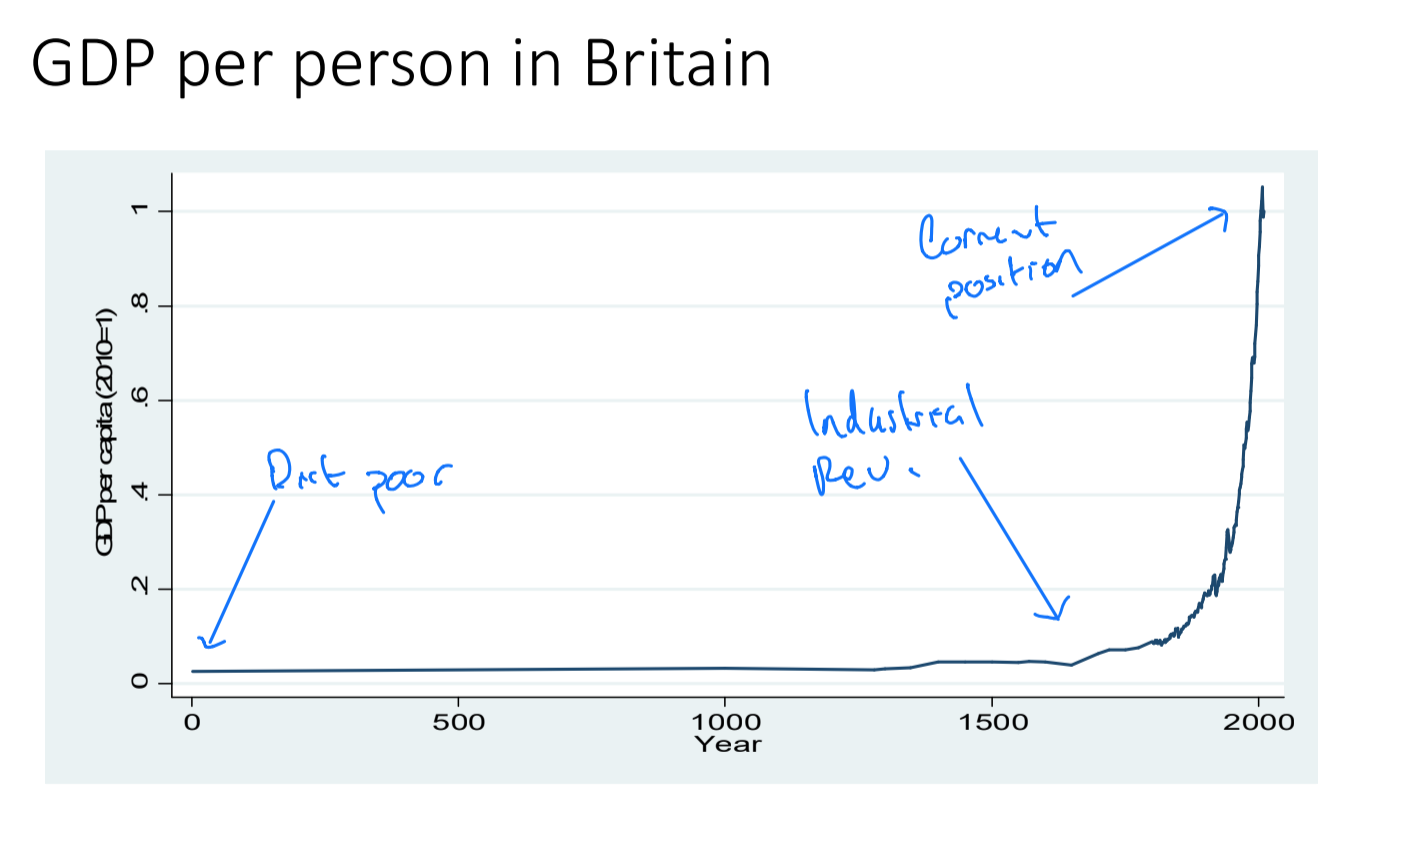
\includegraphics[width=.7\textwidth]{britain_gdp_1}
		\caption{Britain's GDP over time}
		\label{fig:britain_gdp_1}
	\end{minipage}\hfill
	\begin{minipage}{0.45\textwidth}
		\centering
		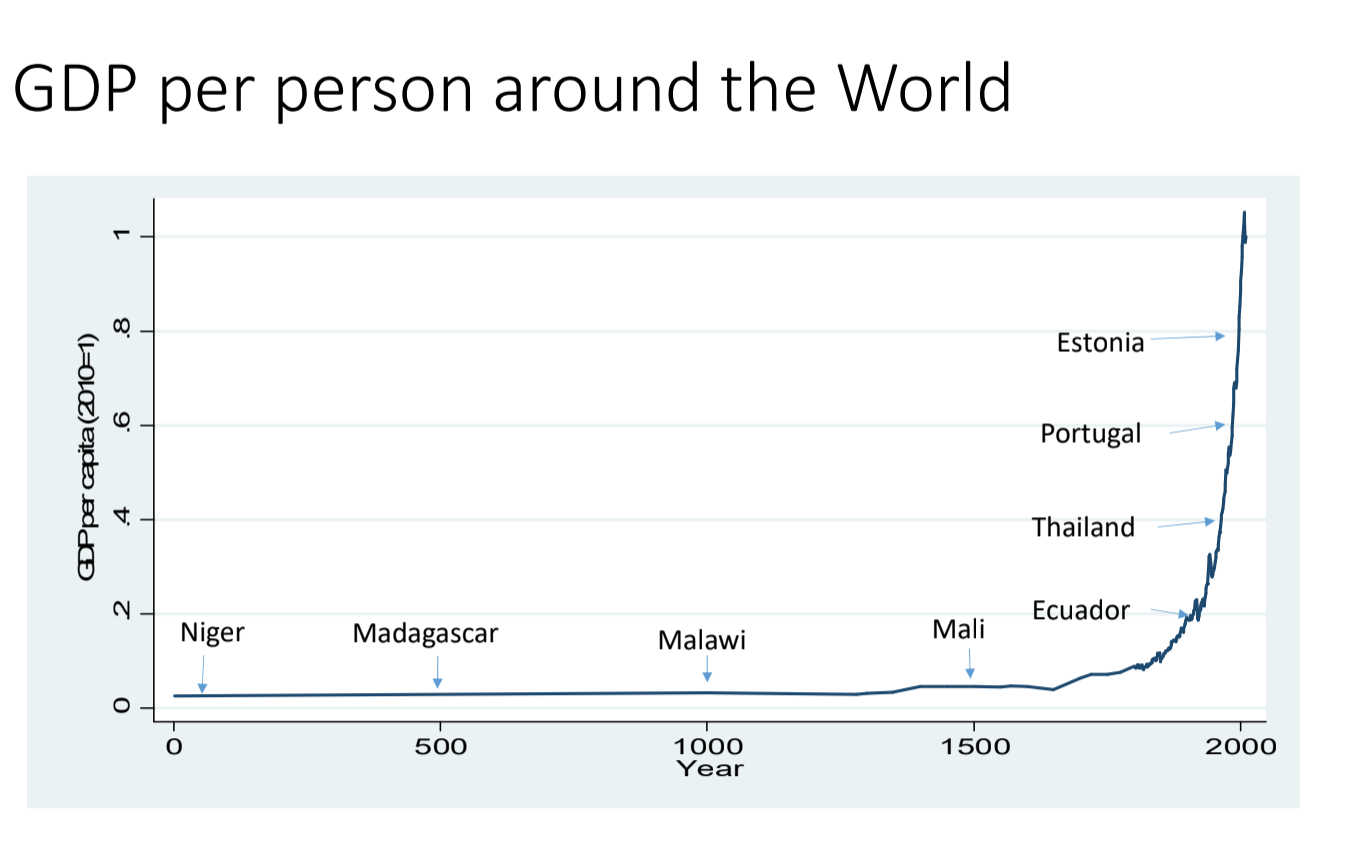
\includegraphics[width=.7\textwidth]{britain_gdp_2}
		\caption{Britain's GDP compared to other countries NOW}
		\label{fig:britain_gdp_2}
	\end{minipage}
\end{figure}	
	
\begin{figure}[h]
	\begin{minipage}{.45\textwidth}
		\centering
		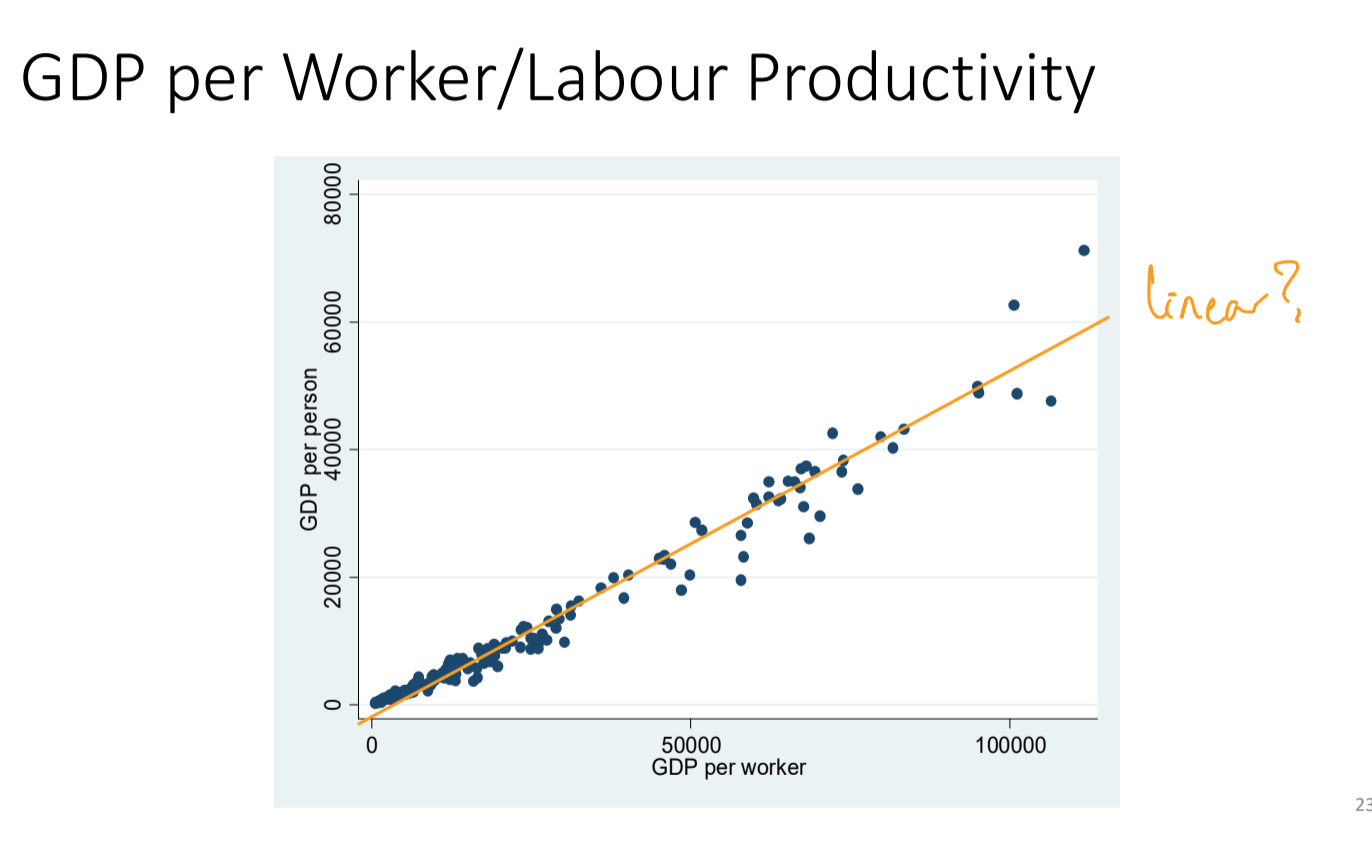
\includegraphics[width=.7\textwidth]{gdp_productivity_1}
		\caption{GDP vs Productivity}
		\label{fig:gdp_productivity_1}
	\end{minipage}\hfill
	\begin{minipage}{.45\textwidth}
		\centering
		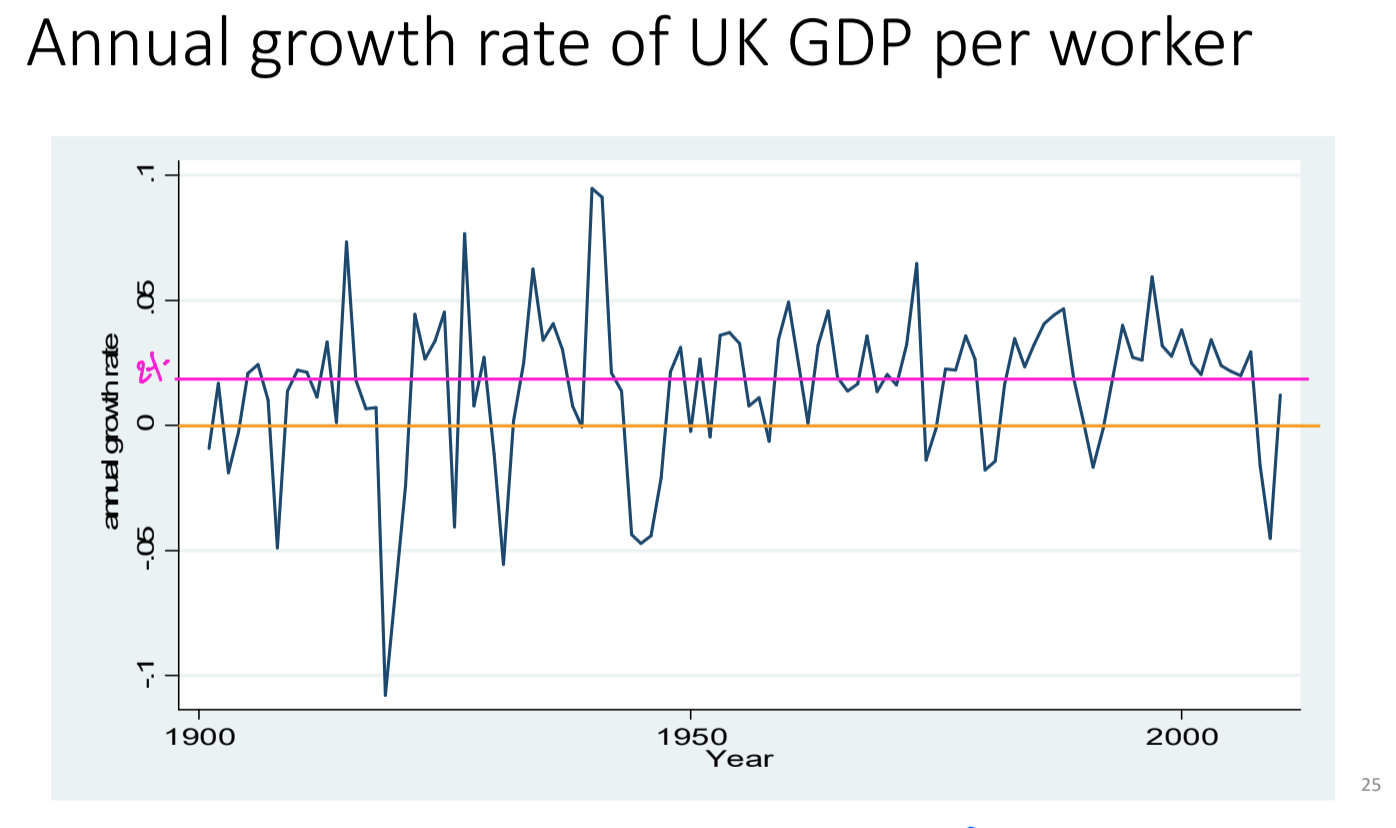
\includegraphics[width=.7\textwidth]{britain_gdp_3}
		\caption{Britain's GDP Growth Trend}
		\label{fig:britain_gdp_3}
	\end{minipage}
	
\end{figure}

\newpage
\section{Growth Engines}
Here we move onto the main drivers for growth in the economy. We will use an analogy of a hunting village, whereby the hunters use arrows to catch their game, to spell out these engines specifically. The engines that we will discuss are as follows:
\begin{itemize}
	\item More arrows per hunter: \textbf{Capital Accumulation}
	\item Better arrows to use: \textbf{Technological Change}
	\item Hunting in a pack: \textbf{Management Quality}
	\item More hunting training: \textbf{Human Capital Accumulation}
\end{itemize}

\textbf{n.b. For this example, we will assume that $Kills/worker = GDP/capita$ and $Kills \; Total = GDP \; Total$}

\subsection{Capital Accumulation}
More arrows per hunter in our analogy is called \textbf{capital} accumulation as we have more productive resources to utilise in our day to day production of game. This is done through the process of \textbf{investment.}

\subsubsection{Definitions}
Beginning with some definitions:
\begin{itemize}
	\item \textbf{Capital:} the stock of equipment and structures at a certain point in time
	\item \textbf{Investment:} the addition toe the stock of equipment and structures
\end{itemize}

\subsubsection{Accumulation and Growth}
The causal mechanism for accumulation and then growth is through how workers use capital. 

Think of capital as \textbf{aids in production to effectively produce more,} like how the arrows in the hunting village help with killing more animals. 

Investment leads to the accumulation of this capital as there will be growth in \textbf{capital per worker,} adding to the overall stock. 

Growth in capital per worker leads to growth in \textbf{GDP per worker} as each worker is more productive.

\subsubsection{Nature of Investment}
The nature of investment is such that there is a sacrifice of current consumption to achieve a greater level of future consumption. Some of the workers and capital are labouring to produce new capital instead of producing goods and services for immediate use.

\subsubsection{Investment in an Open Economy}
We can not sacrifice consumption domestically to gain investment into the economy through the use of imports: \textbf{capital goods are imported whilst domestic workers dedicate themselves to consumption goods.}

However, this implies \textbf{debt accumulation} as you are borrowing funds to pay for these expensive imported capital goods. Since foreign debt cannot be accumulated \textbf{indefinitely,} the consumption sacrifice is only postponed to a later date. This is when there is a requirement to pay off debt. Hence, \textbf{the later sacrifice} meaning that there is still a trade-off between investment and consumption.

\subsection{Technological Change}
Better arrows per hunter is called \textbf{technological change} as we have better productive resources to utilise. \textbf{Note that this does not mean more productive resources.} As we have better resources to use, we are more productive with them. Change happens through \textbf{innovation.}

\subsubsection{Definitions}
Beginning with some definitions:
\begin{itemize}
	\item \textbf{Innovation:} introduction of new ways of doing more with less or the same amount. These efficiency gains are found in the \textbf{production process.} Innovation is usually knowledge shared freely in society.
\end{itemize}

Note that in modern economies, innovation is the outcome of:
\begin{itemize}
	\item Basic research, mostly done in universities
	\item Research and Design \textbf{(R\&D),} mostly done in firms
\end{itemize}

\subsubsection{Economics of R\&D}
There are some key characteristics of innovation that must be recognised to show the thorny parts of R\&D as it can sometimes cause barriers to technological change:
\begin{itemize}
	\item \textbf{Upfront research costs:} Increase the burden of risk as there is a large requirement of upfront capital.
	\item \textbf{Non-Rivalrous:} One person's use does not exclude another person from using it. This means that if one firm creates an idea, without any protection around it, another firm can steal the idea and use it.
\end{itemize}
Hence, without any intervention, the costs for R\&D are too high whilst the benefits are too low. We can see that with an equation below:
\begin{center}
$N = Net\;Benefit$ \\ $R = Reward\;for\;Successful\;R\&D$ \\ $P_R = Probability\;of\;Success$ \\ $C = Cost\;of\;R\&D$ \\ $P_C = Probability\;of\;Idea\;Stolen$
\end{center}
Hence knowing that $P_R$ is low and $P_C$ is high, we have the equation:
\begin{center}
$N = R \times P_R - C\times P_C$ where $N<0$
\end{center}

\subsubsection{Policy Solutions to the R\&D Problem}
Here are some solutions:
\begin{itemize}
	\item Patents:
		\begin{itemize}
			\item Intellectual property rights
			\item Effective creation of monopolies over a certain good or service
			\item Usually lasts 15-20 years
			\item Opportunity for firms to make profit from their R\&D
		\end{itemize}
	\item Subsidies: reduced costs for R\&D ventures conditional on their R\&D performance
\end{itemize}

\subsubsection{Economics of Basic Research}
Basic research is about the type of activity generating positive externalities, \textbf{that is, a positive effect on a third party during the production or consumption of a good or service, in this case \textit{research}.}

In terms of the funding:
\begin{itemize}
	\item Subsidies are given by the government e.g. Economic and Social Research Council (ESRC)
	\item Stimulates research and research proposals
	\item Adds value to the economy without the pricing mechanism in place effectively 'shifting the frontiers of what is possible.'
\end{itemize}

\subsubsection{Technological Change in Poorer Countries}
Imitation makes a lot more sense than innovation in poorer countries. However, the issue is that \textbf{knowledge does not flow that easily.} Limited knowledge leads to a lack of accessibility. Successful imitation, however, shows miraculous levels of growth: \textbf{China and Japan being notable examples}

This issue of information dissemination is because new ideas contain two types of knowledge:
\begin{itemize}
	\item \textbf{Explicit Knowledge:} formulas, blue prints, instructions
	\item \textbf{Tacit Knowledge:} nuanced knowledge like application with certain people etc. which cannot be communicated as effectively.
\end{itemize}

\subsubsection{Sources of International Technology Diffusion}
There exists two main ways of technological change moving around the world:
\begin{enumerate}
	\item Foreign Direct Investment
	\item Trade
\end{enumerate}

\textbf{Foreign Direct Investment (FDI):}
\begin{itemize}
	\item Foreign entity starts or acquires productive resources outside their home country
	\item Direct technology transfer through a literal implementation of the firms technology abroad
	\item Diffusion through imitation clusters, when the technology from an initial investment is taken up by aspiring entrepreneurs
	\item Competition with local, inefficient firms who need to learn/imitate/adapt or be pushed out of the market due to being priced out
\end{itemize}

\textbf{Trade:}\\
In trade there are exports and imports. Both contribute to technology diffusion:
\begin{itemize}
	\item Imports:
		\begin{itemize}
			\item Embodied technology e.g. importing IT systems
			\item Pressure on local inefficient firms to adapt $\rightarrow$ same as FDI
		\end{itemize}
	\item Exports:
		\begin{itemize}
			\item Learning by exporting $\rightarrow$ learn to be more efficient and learn how to adapt to the demands of countries abroad
			\item Market size increases $\rightarrow$ access to a larger market allows for diffusion of technology into developing countries simply because of broader exposure
		\end{itemize}
\end{itemize}

\subsubsection{International Tech Diffusion and IPRs}
\textbf{Question:} Should poorer countries enforce intellectual property rights (IPRs) of rich-country firms?\\
There is a temptation to believe that not enforcing them can lead to cheap production by imitation however possible problems persist:
\begin{itemize}
	\item It discourages FDI as there is no more profitability for these foreign firms to come into the developing market
	\item There would be adverse effects on rich country innovation as there is no longer an incentive to innovate. \textit{This is based on the premise that firms are innovating to conduct FDI}
	\item Rich countries simply do not like it. This might result in a lack of trade and a souring of international relations which can subsequently cause a trade war
\end{itemize}

Yet, even with enforcement, a lack of enforcement could persist anyway due to the negligence of IPRs and Patents in developing countries. Hence, the issue appears to be much more complicated than black or white.

\subsubsection{Embodied Technology}
The distinction between capital accumulation or growth and innovation or imitation is conceptually useful. \textbf{However,} in practice, a lot of innovation or imitation is embodied in capital itself. Thus, the two often come in the same package. Investment is itself a source of technological change.

\subsection{Management Quality}
Management quality drives growth through putting people who are good at the right thing in the right place. This is done through \textbf{specialisation} and \textbf{comparative advantage.} Examples of high management quality:
\begin{itemize}
	\item Adam Smith's pin factory $\rightarrow$ division of labour (specialisation)
	\item Henry Ford's assembly line $\rightarrow$ division of labour as well
	\item Outsourcing and global supply chains $\rightarrow$ utilising comparative advantage
	\item Gig economy $\rightarrow$ workers connecting through an information supply chain with an increased division in labour and level of specialisation
\end{itemize}

\subsubsection{Definitions}
Beginning with some definitions:
\begin{itemize}
	\item \textbf{Specialisation:} focusing on one task and increasing the efficiency at which it is done.
	\item \textbf{Comparative Advantage:} whereby the opportunity cost to produce something for something else/someone is less than another entity. \textit{One would say that a country has a comparative advantage if its opportunity cost to produce is less than another's.}
\end{itemize}

Further to that, organisational change can sometimes come as a form of technical change. You can do more with the same resources and it often requires some upfront R\&D investment. An example would be something like \textbf{software to manage supply chains,} both organisational and technical.

\subsubsection{The Indian Manufacturing Case Study}
To test the real effects of management quality, consulting companies went into India to perform a test whereby control groups of firms were given no management consultants while tested firms were given management consultants to fix their most pressing issues over a few days.

\textbf{Before:}
\begin{itemize}
	\item The manufacturing firms in India were very disorganised with dirty and poorly maintained machinery whilst equipment was lying across the floor. 
	\item Yarn had no labels, order or damp protection. Further, it was piled so high, access was restricted in the factory itself
	\item Poor storage practices also made some stock unusable, requiring further treatment to be used again
\end{itemize}
\textbf{After:}
\begin{itemize}
	\item Stock was organised and labelled
	\item Stock was also tagged and entered into the computer
	\item Factory was cleaned and maintained to a higher standard
\end{itemize}

\subsubsection{Managerial Quality}
Within a country, there is a big disparity in productivity among firms possibly due to the differences in managerial quality as a result of the different levels of organisation. There would be big gains from bringing up efficiency at the tail: \textit{the lower end of the distribution is lagging far behind but can account for a lot of firms within the country.}\\

\textbf{Causes of Poor Managerial Quality:}
\begin{itemize}
	\item Dynastic Management: management of the firm kept within a family, not meritocratic and there is no guarantee of skill or will from future generations
	\item Crony Capitalism: Prevalent in low-income countries. Owners and managers are kept in a tight circle and benefits are accrued through political connections.
		\begin{itemize}
			\item Shareholders can benefit due to their own connections
			\item Productivity will be low due to mostly incapable management $\rightarrow$ again, not meritocratic but based on nepotism
		\end{itemize}
	\item State Owned Enterprises: directly appointed by the government, low productivity due to failed selection process at some points\\
\end{itemize}

\textbf{Entry Costs, Financial markets and Managerial Quality}
\begin{itemize}
	\item Talented outsiders could:
		\begin{itemize}
			\item Buy out incumbents $\rightarrow$ but a lack of capital means they might not be able to, further, they can't judge their own talent compared to the market without experience
			\item Enter with their own startups to compete them out of the market
		\end{itemize}
	\item High entry costs:
		\begin{itemize}
			\item Upfront production costs as capital raising is difficult
			\item Licenses, permits etc. are barriers to entry
		\end{itemize}
	\item Poorly developed financial markets:
		\begin{itemize}
			\item Typically as a result of inefficient contract enforcement
			\item This adds further difficulty to ensuring capital
		\end{itemize}
\end{itemize}
Hence, it is obvious that Managerial Quality can be severely affected by a plethora of other factors. However, its contribution to growth can also be very large, especially at the weaker end of the distribution where basic practices - \textbf{ref: Indian Case Study} - have not even been implemented.

\subsection{Human Capital Accumulation}
More years in hunting school in our analogy translates to human capital accumulation. With more human capital, workers are intrinsically more productive and efficient and can apply their knowledge to technological, capital and managerial change. This is a cumulative effect from education that has knock-on effects on the facilitation of innovation and imitation.

\subsubsection{Definitions}
Beginning with some definitions:
\begin{itemize}
	\item \textbf{Human Capital:} anything embodied in workers which makes them more productive, a form of internal development
\end{itemize}
The greatest focus of policy thus far has been \textbf{schooling} and \textbf{health} which aim to improve a persons ability to live and participate in the economy. Examples of foundations that have helped to develop this are:
\begin{itemize}
	\item The Gates Foundation who aid in Malaria efforts and education
	\item The United Nations who have committees dedicated to raising the standard of living through education and healthcare especially in underdeveloped countries
\end{itemize}

\subsection{Engine Interaction}
We will discuss here how these growth engines interact and whether or not growth can come from a single engine. The latter first:

\begin{center}
\noindent\fbox{\begin{minipage}{.8\textwidth}

\textbf{Ten hunters, 3 permanently on arrow-making duty. Initial endowment of 1 arrow power hunter. Over time, the change in GDP per worker will:}
\begin{enumerate}
	\item Increase
	\item Decrease
	\item Stay constant
\end{enumerate}

\textbf{\textit{Answer is 2.} Decrease due to the diminishing marginal returns on capital.} At some point, producing more capital leads to a plateauing increase in productivity.

\end{minipage}}
\end{center}

Capital accumulation and GDP growth is shown through the average product of capital. This is known by $Average\;Product\;of\;Capital = \frac{GDP\;per\;Worker}{Capital\;per\;Worker}$

In our hunting village example this would translate to $APC = \frac{Deer}{Arrows}$. Gains from additional capital is known as the marginal product of capital which is known by the additional gain to product when there is a \textbf{unit increase in capital.}

\subsubsection{Limits to Growth from Capital Accumulation}
There are definitive limits to simply using investment as a driver for growth:
\begin{itemize}
	\item The average product of capital declines due to the law of diminishing marginal returns
	\item The investment rate has a natural ceiling as it is limited by what is available i.e. it is difficult to invest beyond 100\% of GDP
	\item Capital accumulation alone cannot sustain indefinite growth
\end{itemize}
From this we can see that:
\begin{itemize}
	\item Capital accumulation depresses the average product of capital
	\item Innovation, organisational change and human capital accumulation boost the average product of capital
		\begin{itemize}
			\item Hunting in a pack improves the productivity of all arrows
			\item More trained hunters improve the productivity of all arrows
		\end{itemize}
\end{itemize}
Hence all engines appear to complement one another to ensure that one engine does not depress the average product of capital entirely.

\subsubsection{Engine Complementarity}
\textbf{Technical, organisation change and human capital accumulation keep the average product of capital falling even though capital per worker keeps increasing.}

Although they might depress their own marginal productivity, this is offset by growth in the other engines. Think of the engines as multiplicative instead of additive:
\begin{center}
	$Engine\; 1 + Engine\; 2 + Engine\; 3 + Engine\; 4$
\end{center}

\subsubsection{The Role of the State in Growth}
The State plays a major role in the growth of the economy and they can facilitate it or hinder it depending on their policy. Below are ways in which the State can impact growth:\\

\textbf{Fuel for Engines}
\begin{itemize}
	\item Investment in infrastructure which is a capital good
	\item Subsidies for R\&D and basic research
	\item Investment into education and healthcare with good policy
\end{itemize}

\textbf{Regulation}
\begin{itemize}
	\item Markets for goods and services are regulated by the state dictating what conditions people can operate under
	\item Regulation for labour and financial issues are regulated along the same lines
	\item International trade which is facilitated by the state through free trade or hindered by tariffs and trade wars
\end{itemize}

\textbf{Rule of Law}
\begin{itemize}
	\item Laws to change the operation of companies e.g. GDPR in Europe
	\item \textbf{But} rigidity is also key for smooth business operation as predictability is key to confidence in operations
	\item Implementation of processes we can follow within a reasonable boundary
\end{itemize}

\subsubsection{Corruption and Growth}
Another issue to consider when thinking about growth is corruption. Here are some reasons why:
\begin{itemize}
	\item Saps incentives for innovation, imitation and investment if corrupt officials target successful entrepreneurs. This is due to the burden of bribe payments which means less money to innovate or incentivise productivity.
	\item Creates barriers to entry for outsiders if those inside use corruption to buy protection, privileged treatment or judicial bias which means less incentive to innovate or even try in the first place
	\item Deprives government of funds for infrastructure, education, administration of justice due to embezzlement. This means less investment into the engines of growth within the economy by the government
\end{itemize}

\subsection{Growth Engines: Appendix}
Find related materials here. Some may be repeated from other appendices.
\subsubsection{Formulae and Definitions}
\begin{itemize}
	\item \textbf{Investment Rate:}
		\begin{itemize}
			\item A measure of the sacrifice an economy makes of current consumption for a greater level of future consumption.
			\item \textbf{Formula:} $Investment\;rate = \frac{Level\;of\;investment}{GDP}$
		\end{itemize}
	\item \textbf{Average Product of Capital:}
		\begin{itemize}
			\item The amount of product that you gain from total capital invested into a worker.
			\item \textbf{Formula:} $Average\;Product\;of\;Capital = \frac{GDP\;per\;Worker}{Capital\;per\;Worker}$
		\end{itemize}
	\item \textbf{$\Delta$ in Capital per Worker:}
		\begin{itemize}
			\item The change in capital that a worker has, averaged across the whole economy.
			\item \textbf{Formula:} $\Delta Capital\;per\;worker = investment\; rate \times GDP\;per\;Worker$
		\end{itemize}
	\item \textbf{Growth Rate of Capital per Worker:}
		\begin{itemize}
			\item The growth in capital that a worker has, averaged across the whole economy.
			\item \textbf{Formula:} $Growth\;Rate\;of\; Capital\;per\;worker = investment\; rate \times (GDP\;per\;Worker / Capital\;per\;worker)$
		\end{itemize}
		
\end{itemize}

\newpage
\section{Economic Fluctuations}
This section will dive into the economic fluctuations commonly seen within an economy. There exists two types of fluctuation in the economy:
\begin{itemize}
	\item Aggregate Demand Shocks
	\item Aggregate Supply Shocks
\end{itemize}

These can also be talked about as:
\begin{itemize}
	\item Tailwinds $\rightarrow$ pick up in growth
	\item Headwings $\rightarrow$ shock slowing down rate of growth
\end{itemize}

\subsection{Demand Shocks}
We will first discuss demand shocks in the economy.

\subsubsection{GDP Composition}
Recalling the equation
\begin{center}

$ GDP = C + I + G + (X-M)$

\end{center}

From here we can see the breakdown:
\begin{itemize}
	\item \textbf{(C)onsumption:} goods and services bought by households
	\item \textbf{(G)overnment Spending:} goods and services bought (or produced) by the government
	\item \textbf{(I)nvestment:} investment goods bought by firms
	\item \textbf{(E(x)ports):} goods, services and investment goods sold abroad
	\item \textbf{(I(m)ports):} goods, services and investment goods bought abroad
\end{itemize}

With these we can move on to how this composition can cause the actual shock.

\subsubsection{Aggregate Demand}
Anything that suddenly causes:
\begin{itemize}
	\item A change in government spending \textbf{G}
	\item A change in \textit{desired} investment \textbf{I}
	\item A change in \textit{desired} investment \textbf{C}
	\item A change in net exports \textbf{NX}
\end{itemize}

Following that, we can see some examples of demand shocks:
\begin{itemize}
	\item \textbf{G:}
		\begin{itemize}
			\item Wars $\rightarrow$ planned spending increases due to necessity of building and providing materials
			\item Changes in ideology $\rightarrow$ austerity in government spending, reducing \textbf{G} by a large amount
			\item Fiscal crises, such as Venezuela and hyperinflation and further  Sovereign Debt Crises
		\end{itemize}
	\item \textbf{I and C:}
		\begin{itemize}
			\item Changes in taxes $\rightarrow$ increases in income tax decreases ability to consume while increases in corporate tax will reduce investment - the counter case is probable too
			\item Changes in wealth $\rightarrow$ anticipation in increasing wealth and its tangible effects on how one would spend. If you think you are wealthy, your propensity to spend increases as well
			\item Psychological changes (Keynesian animal spirits) $\rightarrow$ anticipation, proclivities or behavioural reaction that is unpredictable and ultimately reliant on the individual
		\end{itemize}
	\item \textbf{X - M:}
		\begin{itemize}
			\item Changes in exchange rates $\rightarrow$ a result of currency strength
			\item Foreign demand shocks $\rightarrow$ they could reduce or increase exports and imports depending on what the shock is. If it's negative, exports are likely to reduce while imports, due to lower production, might also reduce
		\end{itemize}
\end{itemize}

However, one has to be careful on the causality of aggregate demand shocks on GDP:
\begin{center}
	$GDP = C + I + G + (X-M)$ \\
	This is not a causal relationship
\end{center}
You have to question what makes firms respond to the change in AD as GDP is not simply caused by planned spending. There is a missing step as well that might not be identified in the equation.

\subsubsection{Narrative of the Aggregate Demand Shock}
With the previous in mind, let's construct a narrative to show how an aggregate demand shock actually works:
\begin{enumerate}
	\item Consumers decide to spend 10% more
		\begin{itemize}
			\item They have increased confidence
			\item They have an improved ability to pay
			\item They have an increased level of wealth
		\end{itemize}
	\item This leads to an increase in aggregate demand by 10\% as planned spending has increased
	\item Marginal costs go up
		\begin{itemize}
			\item Marginal costs of production increase
			\item This is through expansion of production due to demand increasing
		\end{itemize}
	\item Prices go up
		\begin{itemize}
			\item Since marginal costs increase, this is translated into price:
			\item $MC > P \therefore\; P\uparrow\; \therefore\; MC\uparrow\; until\;MC = P$ 
		\end{itemize}
	\item Increase is proportional i.e. 10\% increase in prices
		\begin{itemize}
			\item Price increase will match demand increase
			\item Equilibrium is a situation where the economy ends up in after the shock
		\end{itemize}
\end{enumerate}

The price increase matches the demand increase because:
\begin{itemize}
	\item Consumers are happy as they are spending 10\%
	\item Firms are happy as marginal cost is up 10\% as it depends on prices and wages
		\begin{itemize}
			\item Same amount of materials and workers
			\item Wages are 10\% higher as well due to price increase, all
		\end{itemize}
	\item Marginal revenue is up 10\% as it is the price, MR=MC\\
\end{itemize}
\textbf{Lessons from the narrative:} \\ \\
After an aggregate demand shock:
\begin{itemize}
	\item Quantities change in the same direction
	\item Prices (gradually) adjust in the same direction
	\item After prices have adjusted, no effect on quantities, a movement back to its original position
\end{itemize}
The size and duration of effect on quantities depend on speed of price adjustment:
\begin{itemize}
	\item A fast price adjustment has a small impact on quantities
	\item A slow price adjustment has a big impact on quantities
\end{itemize}

We can see that price changes, however, vary heavily between firms. Below is a table of collected data from the University of Chicago by Blinder (1994):
\begin{center}
	\begin{tabular}{c c}
		Frequency & Percentage of Firms\\
		\hline
		Less than one & 10.2\\
		Once & 39.3\\
		1.01 to 2 & 15.6\\
		2.01 to 4 & 12.9\\
		4.01 to 12 & 7.5\\
		12.01 to 52 & 4.3\\
		52.01 to 365 & 8.6\\
		More than 365 & 1.6\\
		\hline
	\end{tabular}
\end{center}
Hence, we can see that the price change which is most popular, \textbf{once,} shows the relatively infrequent changes in price that a firm puts out. It can be argued that due to this low infrequency, the aggregate demand shock is actually absorbed by firms. \\\\
\textbf{Explanations for Price Stickiness}\\
Here are some explanations why prices might not change as frequently as one might think, i.e. in alignment with the \textbf{frequency of aggregate demand shocks} people experience.
\begin{itemize}
	\item \textbf{Menu costs:} there are costs associated to changing the price such as physically having to print new menus
	\item \textbf{Information costs:} there is an opportunity cost of time to get and process information on what the right price to put is
	\item \textbf{Strategic considerations:} perhaps being the first to move on price might be bad, especially increasing, as market share can go down drastically if a lot of other substitutes are in place
	\item \textbf{Wage rigidity:} wages change very rarely, typically yearly, so price adjustment would not fit wages. Wages $\rightarrow$ Demand $\rightarrow$ Prices. Thus rigidity begets rigidity, if prices were to change, consumers might switch or not purchase
\end{itemize}

\subsection{Counter-cyclical Policy}
\textbf{Goals of counter-cyclical policy:}
\begin{itemize}
	\item Counter negative aggregate demand shocks to prevent recessions
	\item Counter positive aggregate demand shocks to prevent excessive inflation
\end{itemize}

There are two main types of counter-cyclical policy:
\begin{itemize}
	\item \textbf{Fiscal Policy:}
		\begin{itemize}
			\item Changes in government spending (including transfers) and taxes
			\item Run by the treasury (though this is country dependent)
		\end{itemize}
	\item \textbf{Monetary Policy:}
		\begin{itemize}
			\item Purchases and sales of financial assets, setting of statutory i.e. required interest rates
			\item Run by the central bank
		\end{itemize}
\end{itemize}

\subsubsection{Fiscal Policy}
Here are some concepts related to \textbf{fiscal policy:}
\begin{itemize}
	\item \textbf{Government Spending:} goods, service bought or produced by the government along with transfers such as benefits and interest paid
	\item \textbf{Government Revenues:} from mostly taxes
	\item \textbf{Deficit:} $Spending > Revenues = \Delta Debt$
	\item \textbf{Surplus:} $Spending < Revenues = -\Delta Debt$ \\
\end{itemize} 
\textbf{Fiscal policy also has a dual role:}
\begin{itemize}
	\item A source of demand shocks: the recent austerity programme in UK
	\item A tool to counter other demand shocks: increase in deficit in recessions to increase spending, fiscal stimulus policies in 2007-2009\\
\end{itemize}
Further to that, there is the concept of the fiscal multiplier: the change in GDP due to a £1 change in the deficit. This multiplier is generally thought to be \textbf{greater than 0 and less than 1.} Below is a sample question:

\begin{center}
\noindent\fbox{\begin{minipage}{.8\textwidth}

\textbf{Suppose the government spending multiplier is less than 1. $C+I+NX$ \_\_\_\_ when G increases:}
\begin{enumerate}
	\item Increases
	\item Decreases
\end{enumerate}

\textbf{\textit{Answer is 2.} Decrease due to GDP remaining constant as $Y = C + I + G + (X-M)$.} This means that $C + I + (X - M)$ will reduce to balance $G$ increasing.

\end{minipage}}
\end{center}
\textbf{Crowing Out:}
However, given the use of fiscal policy, crowding out is also a major issue:
\begin{itemize}
	\item \textbf{Definition:} The crowding out effect is an economic theory arguing that rising public sector spending drives down or even eliminates private sector spending. (Kenton 2019)
	\item Some of the increase in spending mobilises idle resources but some diverts resources from other uses. \textit{The multiplier is larger when there are many idle resources}
	\item Some of the tax cuts are spent on goods and services but some are saved. \textit{The multiplier is larger when people have a large propensity to consume}
	\item Fiscal policy is most effective in severe recessions \textbf{i.e. the multiplier $>$ 1}
\end{itemize}
Hence, crowding out means a reduction in private spending despite the government's initiative to increase spending overall. This is shown by saving from reduced taxation or shifting resources instead of mobilising them. There is minimal crowding out when there are many idle resources but a significant crowding out when significant tax cuts could lead to savings.\\\\
There are limits to \textbf{Expansionary Fiscal Policy:}
\begin{center}
	$Deficit = \Delta Debt$\\
	Deficit adds to the debt:
		\begin{itemize}
			\item If the deficit is $+ve$, $\Delta Debt$ is $-ve$
			\item If the deficit is $-ve$, $\Delta Debt$ is $+ve$
		\end{itemize}
\end{center}
However, note that the deficit is still beneficial in some cases. As we discussed before, the increase in borrowing can be used to fund capital goods that might increase future consumption greatly. Just using debt in moderation is required.

Thus, here are some \textbf{Golden Rules for Fiscal Policy:}
\begin{itemize}
	\item Run a deficit in recession and a surplus during the boom. \textbf{Fiscal Policy should be countercyclical where possible}
	\item \textbf{Balance the budget on average,} this comes from following the previous advice
	\item \textbf{Do not run a balanced budget all the time!} Governments need to know how to be contextual with their balance sheet to promote growth or slow it in anticipation of a recession
\end{itemize}

\subsubsection{Monetary Policy}
We now move onto Monetary Policy. This is seen to be the job of central banks: the Federal Reserve: \textbf{The Fed,} the Bank of England: \textbf{BoE,} the European Central Bank: \textbf{ECB,} the Bank of Japan: \textbf{BoJ} and so on.

Their goals are to \textbf{counter demand shocks} and this is done through:
\begin{itemize}
	\item Monetary policy to affect \textbf{interest rates:} the cost of borrowing and reward for saving
	\item Interests rates then affect Consumption and Investment\\
\end{itemize}
\textbf{Interest Rates:}
\begin{itemize}
	\item Many forms of borrowing exist in the economy
		\begin{itemize}
			\item Firms and Households borrow from banks
			\item Households borrow by using credit cards
			\item Firms and governments borrow from the public by issuing bonds
		\end{itemize}
	\item Interest is the compensation received by the lender from the borrower
	\item The interest rate is the \textbf{per-unit-value} compensation
\end{itemize}
Interest rates also tend to move together such that if the interest rate on one form of borrowing goes up, interest rates on other forms of borrowing tend to go up as well. Here are some examples:
\begin{itemize}
	\item Interest rate on government bonds go up
	\item Demand for corporate bonds go down
	\item Interest rates on corporate bonds go up
\end{itemize}
From above, if LSE is paying $x\%$ interest and the government is paying $(x+1)\%$ interest, borrowers have the option to arbitrage unless the lender sees this disparity.\\
\textbf{What is a Central Bank?}
The central bank is mainly two things:
\begin{itemize}
	\item The commercial banks' bank, existing as a regulatory institution
		\begin{itemize}
			\item Offers deposits to commercial banks (bank reserves) $\rightarrow$ like a current account for the bank itself
			\item Lends to commercial banks (discount window, repos etc.) $\rightarrow$ loans from the central bank like overdraft, drawing from a credit line
		\end{itemize}
	\item Monopoly supplier of legal tender $\rightarrow$ preserving and regulating the value of money, having the technology to create legal tender that is unforgeable\\
\end{itemize}
\textbf{Policy Rates}
The central bank has a crucial role in setting the policy rates:
\begin{itemize}
	\item Policy rates are interest rates set directly by the central bank
		\begin{itemize}
			\item Rates on bank reserves
			\item Rates on loans to commercial banks
		\end{itemize}
	\item By changing policy rates, central banks can affect all other rates in the economy
\end{itemize}
An example of how this widespread effect works is done below:
\begin{center}
\noindent\fbox{\begin{minipage}{.8\textwidth}
Take the bank's current policy rate to be $x\%$. In the case that the bank decides to reduce this interest rate to $(x-2)\%$, we will see that the interest rate on central bank loans goes down. Financing for commercial banks becomes cheaper as it is effectively cheaper to borrow since the interest payment required is less. This means that commercial banks require lower interest rates to lend to firms and households.
\end{minipage}}
\end{center}
Having had a look at the policy rates, let's see the interactions policy rates have with components of GDP:
\begin{itemize}
	\item Interest rates and \textbf{I:}
		\begin{itemize}
			\item Cash-poor firms: cost of borrowing since high interest means higher costs of debt and low interest means cheaper cost of debt
			\item Cash-rich firms: opportunity cost since high interest provides incentive to lend to make cash and low interest means an opportunity to invest elsewhere for higher returns, potentially their own company
		\end{itemize}
	\item Interest rates and \textbf{C:}
		\begin{itemize}
			\item Cash-poor individuals: cost of borrowing since high interest means higher costs of debt and low interest means cheaper cost of debt e.g. purchasing a house
			\item Cash-rich individuals: uncertain of the borrowing aspect but potentially used to invest in different areas
		\end{itemize}
\end{itemize}
\subsubsection{Economic Activity and Policy}
\textbf{Natural Level of Economic Activity:} the level to which the economy gravitates back after a shock. Price adjustment makes sure that this happens. There is a center of gravity that economy tends to due to the refined outlook people have after a shock. Look at the below picture to understand the fluctuation and \textbf{natural level} the economy gravitates back to:
\begin{center} % Remember to fix the control points for this picture or find a solution to create an oscilliation along a trendline
	\begin{tikzpicture}
		\coordinate (A) at (-3.5, 0);
		\coordinate (B) at (-3.5, 4);
		\coordinate (C) at (3.5, 0);
		\draw (A) -- (B);
		\draw (A) -- (C);
		\coordinate (Start) at (-3.5, 1);
		\coordinate (End) at (3.5, 3.5);
		\draw (Start) -- (End);
		% \draw (Start) .. controls (-2.5, 1.5) and (-1.5, .75) and (0, 2.5).. (End);
	\end{tikzpicture}
\end{center}
\textbf{Counter-Cyclical Monetary Policy}\\
Examples of this type of policy is shown below:
% Go to the lecture to find out the significance of the counter-cyclical policy
\begin{itemize}
	\item Lower interest rates when contractionary aggregate demand shocks take the economy below the natural rate of economic activity
	\item Increase interest rates when expansionary aggregate demand shocks take the economy above the natural rate
\end{itemize}
However, this policy is very difficult to implement. This is because it is very hard to tell whether the economy is \textbf{at, below or above the natural rate of activity.} Further to that, policy mistakes have a real risk:
\begin{itemize}
	\item Monetary (and fiscal) \textbf{expansions generate inflation when the economy is at or above the natural rate of output,} or when they push the economy above the natural rate
	\item Monetary (and fiscal) \textbf{contractions cause recessions when the economy is at or below the natural rate of output,} or when they push the economy below the natural rate\\
\end{itemize}
\textbf{The Effective Lower Bound}\\
To add further complexity to interest rates, we will discuss the effective lower bound.\\
\textbf{Definition:} The point at which interest rates will stop having a tangible effect and the rate below which it is difficult to go.

Before we go into explaining the complexities of it, here are some key terms to recognise:
\begin{itemize}
	\item \textbf{Negative Interest Rates:} incentive to borrow and hoard cash at a very negative point of interest
	\item \textbf{Minimum Interest Rate (ELB):} cost of storing cash exceeds the gains from borrowing and hoarding cash
\end{itemize}
Hence, when interest rates are at the ELB, conventional monetary policy becomes unfeasible as people are not hoarding cash due to storage costs but are not willing to spend anything either. Until recently it was thought that the ELB was 0, also known as the Zero Lower Bound (ZLB) but empirical evidence has shown that Central Banks can go lower, a little into negative interest rates, to stimulate spending. Examples include:
\begin{itemize}
	\item Japan at $-1\%$
	\item Sweden at $-.75\%$
	\item ECB at $-.4\%$
\end{itemize}
There are ways of getting around the effective lower bound such as:
\begin{itemize}
	\item Abolishing paper currency and predominantly using debt cards etc. $\rightarrow$ lose on negative interest rates in deposit account, this would not work on cash as it is tangible, unable to borrow or store notes and coins which means no storage and hoarding of money
	\item Abolishing large denominations $\rightarrow$ storage space required increased as a result of only small denominations existing which increases the cost of handling cash
\end{itemize}
Thus, the effective lower bound is % conclude from lecture notes and online notes

\subsubsection{Unconventional Monetary Policy}
This brings us to our discussion on unconventional monetary policy, sometimes labelled as \textbf{Quantitative Easing:} purchasing a large amount of long-dated bonds to inject money into the economy to stimulate it.

To understand how this works, we will first need to understand the complexities of a bond:
\begin{center}
	\noindent\fbox{\begin{minipage}{.8\textwidth}
		\textbf{Key facts about Bonds:} 
		\begin{itemize}
			\item Simply a vehicle through which one can borrow money
			\item They can be issued by the government or firms. 
			\item Bonds issued by the government are usually labelled as \textbf{risk free bonds.} 
			\item The bond purchaser pays, known as the \textbf{lender.} 
			\item The issuer of the bond, such as the government or firm, is known as the \textbf{borrower,} and is committed to paying coupons of interest payments during the time to maturity.
			\item The time to maturity is the time taken for the bond to be fully repaid and can vary wildly from months to up to 30 years i.e. the time taken to repay the initial lump-sum amount
			\item At the time of maturity, the lender will be paid a certain amount of interest on top of the initial lump-sum that they would be given back at the beginning of the bond issue.
	\end{itemize}
	\end{minipage}}
\end{center}
And on top of that, a bit of financial terminology through looking at the \textbf{Yield Curve} which is presented by a simple picture below:
\begin{center}
\begin{tikzpicture}
	\coordinate (A) at (-3.5, 0);
	\coordinate [label=left:$Interest\;Rate$] (B) at (-3.5, 4);
	\coordinate [label=below:$Maturity$] (C) at (3.5, 0);
	\draw [thick, ->] (A) -- (B);
	\draw [thick, ->] (A) -- (C);
	\coordinate (Start) at (-3.5, 1);
	\coordinate [label=right:$Y_1$] (End) at (3.5, 3.5);
	\draw (Start) -- (End);
\end{tikzpicture}
\end{center}
It slopes up because of the concept called \textbf{Liquidity Premium:} where lenders require extra compensation for locking money in $\rightarrow$ no access in case of emergency or opportunity, unless sold on secondary markets.

Now, establishing our yield curve, we can begin to analyse how the central bank can affect it with \textbf{conventional monetary policy.} This is done through policy rates which affect the most shortest of terms such as deposits, which can be taken out at any time and interbank loans which typically last one or two days. Thus if the central bank lowers policy rates, we can see the shift in the yield curve below:
\begin{center}
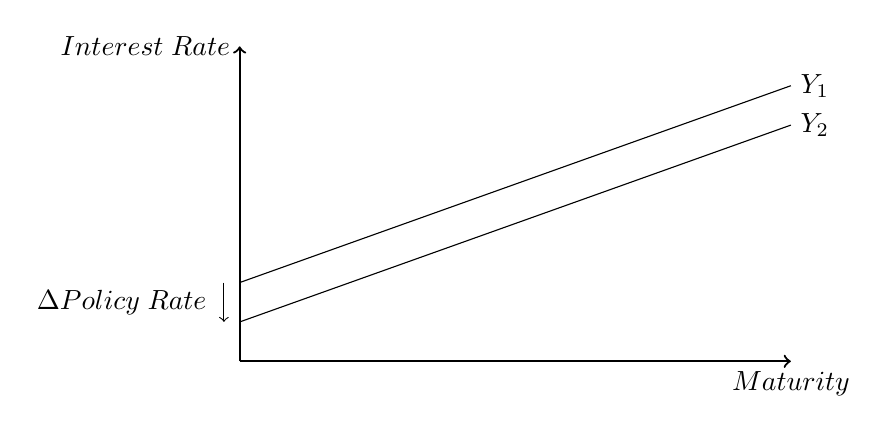
\begin{tikzpicture}
	\coordinate (A) at (-3.5, 0);
	\coordinate [label=left:$Interest\;Rate$] (B) at (-3.5, 4);
	\coordinate [label=below:$Maturity$] (C) at (3.5, 0);
	\draw [thick, ->] (A) -- (B);
	\draw [thick, ->] (A) -- (C);
	\coordinate (Start) at (-3.5, 1);
	\coordinate [label=right:$Y_1$] (End) at (3.5, 3.5);
	\draw (Start) -- (End);
	\coordinate (Start_2) at (-3.5, .5);
	\coordinate [label=right:$Y_2$] (End_2) at (3.5, 3);
	\draw (Start_2) -- (End_2);
	\draw [->] (-3.7, 1) -- (-3.7, .5);
	\coordinate [label=left:$\Delta Policy\;Rate$] (Middle) at (-3.8, .75);
\end{tikzpicture}
\end{center}
Since policy rates are very short term, the maturity is right next to the origin. Further, knowing that interest rates move together, we see a shift downwards at all maturities following this trend. However, this is not the problem we are facing at the ELB. What we are seeing at the ELB is an inability to change the policy rates as shown below:

\begin{center}
\begin{tikzpicture}
	\coordinate (A) at (-3.5, 0);
	\coordinate [label=left:$Interest\;Rate$] (B) at (-3.5, 4);
	\coordinate [label=below:$Maturity$] (C) at (3.5, 0);
	\draw [thick, ->] (A) -- (B);
	\draw [thick, ->] (A) -- (C);
	\coordinate (Start) at (-3.5, 0);
	\coordinate [label=right:$Y_1$] (End) at (3.5, 2.5);
	\draw (Start) -- (End);
\end{tikzpicture}
\end{center}
As shown in the picture above, there is no scope to change the policy rate as it is at the ELB. Thus, unconventional monetary policy aims to flatten the yield curve by dragging it down directly at the later maturities to push the yield curve to a new position as shown below:
\begin{center}
\begin{tikzpicture}
	\coordinate (A) at (-3.5, 0);
	\coordinate [label=left:$Interest\;Rate$] (B) at (-3.5, 4);
	\coordinate [label=below:$Maturity$] (C) at (3.5, 0);
	\draw [thick, ->] (A) -- (B);
	\draw [thick, ->] (A) -- (C);
	\coordinate (Start) at (-3.5, 0);
	\coordinate [label=right:$Y_1$] (End) at (3.5, 2.5);
	\draw (Start) -- (End);
	\coordinate (Start_2) at (-3.5, 0);
	\coordinate [label=right:$Y_2$] (End_2) at (3.5, 1.5);
	\draw (Start_2) -- (End_2);
	\draw [->] (3.7, 2.3) -- (3.7, 1.75);
\end{tikzpicture}
\end{center}
This works through our relationship between Bond Purchases and Interest Rates:
\begin{itemize}
	\item Interest rates fall if demand for bonds exceeds supply $\rightarrow$ this is because more people want to lend money thus those borrowing can bargain for a lower interest rate
	\item Interest rates increase if supply of bonds exceeds demand $\rightarrow$ this is because more people want to borrow money thus those lending can bargain for a higher interest rate
\end{itemize}
Since the central bank is taking bonds out of the market, they artificially cause the supply to fall relative to demand. This makes interest rates fall as we have argued above which makes it easier to borrow. Since interest rates effectively fall down, this affects consumption and investment, stimulating them and subsequently the economy.

However, as a result of this, a lot of central banks balance sheets have exploded due to the amount of long-dated assets that they now hold. To affect interest rates, one must remember that you need to deal in the billions and trillions to move rates around. \textbf{The question of how the central banks will get rid of these assets remains.}\\\\

\textbf{Does Quantitative Easing Work?}\\
Compared to conventional monetary policy, the data available for QE is basically non-existent. However, the effects of QE have definitely placed us in a better position than what we would have been. Not only in economic terms but the uplift in supply of money in the system also provided a psychological boon that prevented our mindsets to go into a deeper recession. Therefore the answer is: \textit{Who knows? But it's better than nothing.}

\subsection{Supply Shocks}
Now we move onto the topic of Supply Shocks. This is any shock in the economy to do with the supply side such, usually production.

\subsubsection{Examples of Supply Shocks}
We will begin with some examples:
\begin{itemize}
	\item Accelerations or decelerations in technical change $\rightarrow$ technological change at a rate that is vastly different to the standard level of technological change can lead to large efficiency gains in production providing a supply shock
	\item Changes in the costs of materials $\rightarrow$ costs which are passed onto production, such as oil, can implicitly control the level of supply as they are inputs into production. Firms have to decide on the level of supply they want to produce and the costs of these inputs impacts them greatly
\end{itemize}

\subsubsection{Supply Shocks and Prices}
Supply shocks have the opposite implications to demand shocks. When there is an expansionary supply shock, there tends to be a fall in prices as costs of production are usually decreasing. When it's contractionary, prices tend to increases as costs of production increase as well. Quantity and prices move in the opposite direction from a supply side perspective. If the quantity of supply increases, prices tend to fall \textbf{note that this is already different from demand.}\\

Further, supply shocks add to the central banks' dilemmas:
\begin{itemize}
	\item One cannot tell where the economy is relative to the natural rate when the supply shock occurs
	\item Contractionary supply shocks reduce quantity and increase price, seen to be the worst of both worlds
	\item Demand cannot be boosted by reducing interest rates as price levels will be exacerbated
\end{itemize}
An example to illustrate this dilemma is when a contractionary supply shock is misdiagnosed as a contractionary demand shock. An attempt at expansionary fiscal policy will have the average price level of goods shooting through the roof.

\subsubsection{The Relative (UN)Importance of Supply Shocks}
Yet, supply shocks do not seem to matter as much and here are some examples why:
\begin{itemize}
	\item Implausibility of technological regress $\rightarrow$ we don't forget the progress that aids production
	\item Many cycles with no clear shock to material prices $\rightarrow$ theres an inability to identify absolute causes to shocks
	\item Prices are procyclical on average $\rightarrow$ prices move usually in the same direction of the cycle while supply shocks are counter-cyclical
\end{itemize}

\subsection{Economic Fluctuations: Appendix}
Find related materials here. Some may be repeated from other appendices.
\subsubsection{Formulae and Definitions}
\begin{itemize}
	\item \textbf{GDP:}
		\begin{itemize}
			\item The amount of goods and services produced in an economy in a year.
			\item \textbf{Formula:} $GDP = C + I + G + (X-M)$
		\end{itemize}
	\item \textbf{Deficit:}
		\begin{itemize}
			\item When government spending exceeds government revenues.
			\item \textbf{Formula:} $-\Delta Deficit = Spending - Revenue$
		\end{itemize}	
	\item \textbf{Surplus:}
		\begin{itemize}
			\item When government revenues exceeds government spending.
			\item \textbf{Formula:} $+\Delta Deficit = Spending - Revenue$
		\end{itemize}	
\end{itemize}


\newpage
\section{Inflation and Deflation}
Now we begin on the topic of inflation with some \textbf{definitions:}
\begin{itemize}
	\item \textbf{Inflation:} the sustained increased in the level of prices
	\item \textbf{Inflation Rate:} the percentage change in the level of prices
	\item \textbf{Consumer Price Index:} measures the cost of buying a representative bundle of consumer goods and services year on year
	\item \textbf{Hyperinflation:} when inflation exceeds $50\%$ per month
	\item \textbf{Deflation:} the sustained decreased in the level of prices, where people are spending less in the economy with the expectation of further price drops
\end{itemize}
\subsection{Inflation}
We will begin with moderate levels of inflation. A key example of moderate inflation would be the \textbf{United Kingdom.}
\subsubsection{Absolute versus Relative Prices}
We will begin with some conceptual groundwork:
\begin{itemize}
	\item \textbf{Absolute price} changes are merely a change in the units of measurement $\rightarrow$ if there is a 10\% absolute price change, everything will be 10\% more expensive
	\item \textbf{Relative price} changes convey information on scarcity or abundance and likes or dislikes $\rightarrow$ scarcity or abundance of one thing relative to another will change its relative price i.e. if something is particularly scarce, its price will increase, if something is liked a lot, then its price will increase relative to other goods and services
\end{itemize}
We want relative prices to tell producers what to do so that resource allocation is optimised in a way.

Hence, inflation is a problem not because it changes absolute prices, if that were the case, everyone would still have the same purchasing power as all things, including wage, increases simultaneously. It is because of changes in real or perceived relative prices that inflation can be problematic. \textbf{It interferes with the information contained within relative prices.}

\subsubsection{Inflation and Relative Prices}
Inflation forces firms to change their price. This might be due to costs of wages increasing or costs of raw materials increasing. Remembering that the frequency of price changes are different from firm to firm, this creates a relative price change as they do not change simultaneously. \textbf{Relative prices then reflect timing of firms' decisions rather than on scarcity/abundance or like/dislike} $\rightarrow$ this creates an inflationary environment that does not send signals related to our previous factors. Firms are forced to change prices when they get a chance messing up our information contained within prices.
\begin{center}
\noindent\fbox{\begin{minipage}{.8\textwidth}
	\textbf{Example:} A firm issues a new catalog each January. As the general price level rises throughout the year, the firm's relative price will fall.
\end{minipage}}
\end{center}
The above is called a \textbf{real relative change in price.}\\

This means that consumers and firms may also mistake absolute price changes for relative price changes. This is not a real relative change!
\begin{center}
\noindent\fbox{\begin{minipage}{.8\textwidth}
	\textbf{Example:} Consumers may feel their purchasing power is falling when it is not. There is a mental disconnect between their own wage increase and the absolute increase in prices. They think themselves as poorer when they are not which is a hit to their welfare, a direct negative psychological effect.
\end{minipage}}
\end{center}
It makes people unhappy and it makes them decide on things incorrectly like cutting their consumption even though their purchasing power has remained the same. Hence, the allocation of resources is adversely affected.

\subsubsection{Inflation and Uncertainity}
The higher the inflation rate, the more variable and unpredictable it becomes i.e. \textbf{increased volatility.}
\begin{itemize}
	\item Higher uncertainity, so risk-averse people are worse off $\rightarrow$ there is a social cost and direct psychological cost inlaid within this
	\item Risk averse people forego potentially profitable opportunities $\rightarrow$ consumption and investment are likely to be reduced
	\item More time, resources and efforts are devoted to financial planning $\rightarrow$ this means that resources are diverted away from better productive activity just to plan ahead, a simple misallocation of resources
\end{itemize}
Here is an example of this variability:
\begin{center}
\noindent\fbox{\begin{minipage}{.8\textwidth}
\textbf{The Inflation Scenario:}\\\\
Two scenarios:
\begin{enumerate}
	\item Inflation at $2\%$ has a probable range of $1\%\;to\;3\%$
	\item Inflation at $10\%$ has a probable range of $6\%\;to\;14\%$
\end{enumerate}
This means a large variability in the range of inflation. Using the example of lending money where we charge a $3\%$ premium on the loan so if inflation is at $0\%$ we charge $3\%$, if inflation is at $5\%$ we charge $8\%$ and so on. So if we have a loan with inflation at $10\%$, we get a premium of $13\%$. \\

However, noting our variability from above, we might be losing out in purchasing power by $1\%$, getting back less from our loan, if inflation goes to $14\%$. Hence, the risk averse would not decide to invest or consume as much in a high inflation market.
\end{minipage}}
\end{center}

\subsubsection{Benefits of Moderate Inflation}
Here are some benefits to consider:
\begin{itemize}
	\item Stay away from deflation which is an insidious problem!
	\item Stay away from the ELB by putting up higher interest rates at normal times which means we are further away from the ELB and more able to rachet down if required
\end{itemize}
Note that $0\%$ inflation means that on average, half the time we are in $-ve$ inflation which could lead to persistent deflation in the future. We are aiming for something a bit higher, a lot of Central banks target around $2\%$.

\subsubsection{Bringing Inflation Down}
\textbf{Question:} why are Central Banks so anxious about having inflation above their target number?\\
\textbf{Answer:} it is very costly and difficult to bring inflation back down.\\\\
Inflation has a major impact on people's forward looking pricing decisions. When producers set prices, they need to get right their forecast. If they are lower than actual inflation, that is costly to them. If they set it higher, their goods and services would become uncompetitive.

If you're coming from 4/5 years of high inflation, you'll naturally expect high inflation the next year. Hence, this expectation might become self-fulfilling. Prices are set $10\%$ higher, wages are asked to be $10\%$ higher etc. Inflation is baked into the forward looking pricing decisions i.e. it is the \textbf{expectation or the norm.}

\textbf{Argentina is stuck in this situation.} This is why Central Banks are worried about these inching upwards of inflation rates. The solution to this issue is to engineer a recession with a \textbf{sharp increase in interest rates.} However, this is a very costly method $\rightarrow$ political upheaval, unemployment in crazy numbers and psychological damage.

\subsubsection{Inflation Targets}
This shows that expectations are incredibly important to success. The most successful Central Banks are those who know how to manage expectations. One method of managing expectations and creating credibility is the public announcement of inflation targets. Here are a couple examples:
\begin{itemize}
	\item Bank of England (BoE): $2\%$ inflation target
	\item European Central Bank (ECB): $<2\%$ inflation, very close to $2\%$
\end{itemize}
These inflation targets are a very clear deal that is made with the public. Even with the fluctutations around it, the trend is around $2\%$.

\subsection{Hyperinflation}
Knowing our standard definition: inflation which exceeds $50\%$ each month, we can know discuss the consequences of Hyperinflation:
\begin{itemize}
	\item Relative prices lose all meaning
	\item Planning is impossible because the future value of money is too uncertain and variable
	\item There is a focus on protecting purchasing power where nearly all effort goes towards $\rightarrow$ daily routine involved running to get groceries when getting paid twice a day, even a minute makes a difference to purchasing power
	\item Production declines as a result of this distracted activity
\end{itemize}

\subsubsection{What Causes Hyperinflation?}
Here is the causal explanation:
\begin{itemize}
	\item Hyperinflation is caused by excessive currency creation
	\item Government printing money causes the price level to rise
	\item If money is printed rapidly enough, the result is hyperinflation
\end{itemize}
Below are a few examples of hyperinflation:
\begin{center}
\begin{tabular}{||c|c|c|c||}

\hline
Country & Period & CPI Inflation (\%) & Money Supply Growth (\%)\\
\hline
Israel & 1983-85 & 338\% & 305\%\\
\hline
Brazil & 1987-94 & 1256\% & 1451\%\\
\hline
Bolivia & 1983-86 & 1818\% & 1727\%\\
\hline
Ukraine & 1992-94 & 2089\% & 1029\%\\
\hline
Argentina & 1988-90 & 2671\% & 1583\%\\
\hline
DRC & 1990-96 & 3039\% & 2373\%\\
\hline
Angola & 1995-96 & 4145\% & 4106\%\\
\hline
Peru & 1988-90 & 5050\% & 3517\%\\
\hline
Zimbabwe & 2005-07 & 5316\% & 9914\%\\
\hline

\end{tabular}
\end{center}
\textbf{What causes excessive money printing?}
\begin{itemize}
	\item Large budget deficits $\rightarrow$ where government spending is far greater than government revenue
	\item No room or political will for fiscal adjustment $\rightarrow$ can't reduce government spending and can't increase taxes
	\item No access to capital markets $\rightarrow$ international lack of confidence in the economy
\end{itemize}

\subsubsection{Ending Hyperinflation}
Here are some ways in which one can reduce hyperinflation:
\begin{itemize}
	\item Fiscal Reform
	\item Monetary Reform
\end{itemize}
\textbf{Fiscal Reform}\\
Government has to become less dependent on money printing. This can be done thorugh fixing the deficit by reducing the large disparities present by introducing higher taxes and lower government spending. Possibly, the ability to attain funding from abroad might be a solution as well.\\\\
\textbf{Monetary Reform}\\
The government can make sure that there is a fixed rate of Money Supply growth. This will change \textbf{expectations,} a key factor, in line with reduced growth. However, this is not observable to people hence it is hard to be fully credible. Further to that, you can set an \textbf{inflation target} which will show some sense of credible commitment. However, this is also a statistic as well which is produced by the government. If the government has no credibility then it would not work out as well. A lot of successful cases of solving hyperinflation happens through a pegging of the currency. Here there is a credible commitment to keeping the currency's value $\rightarrow$ if you print too much, the currency depreciates, if you print too little, it appreciates. This is a tangible and observable change so credible commitment is present.\\\\
\textbf{Central Bank Independence}\\
This is also another solution to ending hyperinflation. This is to provide \textbf{operational independence} which isolates monetary policy from fiscal policy. For example, \textbf{Venezuela's Central Bank is not independent.} Yet, the government still decides the overall framework of what the Central Bank will do. Just the day to day decisions are not interfered with by the government.

\subsection{Deflation}
Now we begin an overview of deflation. Here are the key concerns with deflation:
\begin{itemize}
	\item It causes an incentive for consumers to \textbf{delay purchases} as prices are expected to fall in the future $\rightarrow$ if the consumer does not have an immediate need, they can delay their purchase to save
	\item Further, it can increase debt burdens as the value of money is depreciating while the value of debt is more $\rightarrow$ this makes debt more expensive to pay
	\item Both can exacerbate recessions and lead to a vicious cycle
		\begin{center}
			Recalling our equation $Y = C + I + G + (X-M)$, consumption, through consumers holding back purchases, and investment, through debt becoming more expensive, is likely to fall as a result of deflation
		\end{center}
\end{itemize}

\subsubsection{Fighting Deflation}
The solution seems simple: print lots of money. This:
\begin{itemize}
	\item Decreases the value of money
	\item Induces reasoning to spend now rather than later before value of money is reduced too much
\end{itemize}

\subsection{Inflation and Deflation: Appendix}
Find related materials here. Some may be repeated from other appendices.

\newpage
\section{Unemployment}
The concept of unemployment is central to living standards. This is associated not just with income but psychological and social well-being as it provides a sense of security and purpose. We begin with some key concepts in unemployment:
\begin{itemize}
	\item \textbf{Employed:} working at a paid job
	\item \textbf{Unemployed:} not working but actively looking for a job
	\item \textbf{Labour Force:} all employed and unemployed perople, these are those who are already active or willing to work
	\item \textbf{Rate of Unemployment:} the percentage of the labour force that is unemployed
\end{itemize}
Observations show that:
\begin{itemize}
	\item The unemployment rate is \textbf{counter-cyclical} $\rightarrow$ it rises when there is a recession and falls when there is a boom
	\item The long-run average varies a lot from country to country
\end{itemize}
We also have the concepts of \textbf{Cyclical} and \textbf{Natural} unemployment:
\begin{itemize}
	\item Natural Rate of Unemployment (NRU): the normal unemployment rate the economy experiences when it is neither in a recession nor a boom
	\item Cyclical Component: the difference between the actual and the natural rate $\rightarrow$ the cyclical rate fluctuates away from the NRU due to shocks which are deviations from the norm
\end{itemize}
Therefore, that takes us to our analysis of unemployment. Our previous discussion of economic fluctuations helped us understand the cyclical component. This section will focus on what determines the NRU and ask why it varies across countries.

\subsection{A Basic Model of the NRU}
Through Chris Pissarides, a Nobel Prize Winner, we can model the natural rate.
\begin{center}
	Lets begin with the components of the model:
	\begin{itemize}
		\item $L$ = Number of workers in labour force (fixed)
		\item $E$ = Number of employed workers
		\item $U$ = Number of unemployed workers
	\end{itemize}
	\textbf{Unemployment rate:} $\frac{U}{L}$
\end{center}

\subsubsection{Labour Market Flows: Separations}
This flow shows employment to unemployment. Reasons causing this could be as follows:
\begin{itemize}
	\item Dismissals, redundancies or firm closures $\rightarrow$ firm side
	\item Quits $\rightarrow$ worker side
\end{itemize}
For separations, we have the rate of job separation:
\begin{center}
	$s = rate\;of\;job\;separation$\\
	This is the fraction of employed workers that become separated from their jobs in a given period e.g. $s = 1\%$ per month
\end{center}
\textbf{This is FLOW 1.}

\subsubsection{Labour Market Flows: Matches}
This flow shows unemployment to employment. Conceptually:
\begin{itemize}
	\item Search for workers as firms $\rightarrow$ matches from the firm side
	\item Search for firms as workers $\rightarrow$ matches from the worker side
	\item \textbf{This whole process takes time and effort}
\end{itemize}
\begin{center}
	$f = rate\;of\;job\;finding$\\
	This is the fraction of unemployed workers that find jobs in a given period e.g, $f = 20\%$ per month
\end{center}
\textbf{This is FLOW 2.}

\subsubsection{Transitions between Employment and Unemployment}
From above, we can put \textbf{FLOW 1} and \textbf{FLOW 2} into a simple visual model.
\begin{center}
	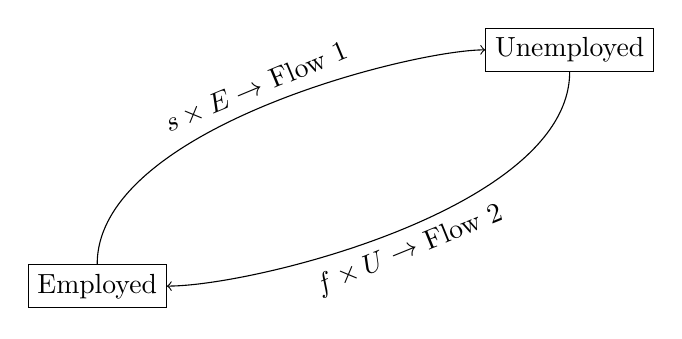
\begin{tikzpicture}
		% Coordinate -3 and Coordinate +3
		\path (-3,0) node[rectangle, draw](E){Employed}
		(3,3) node[rectangle, draw](U) {Unemployed};
		\draw [->](U) .. controls +(down:2cm) and +(right:2cm) .. node[below, sloped] {$f\times U \rightarrow$ Flow 2} (E);
		\draw [->](E) .. controls +(up:2cm) and +(left:2cm) .. node[above, sloped] {$s\times E \rightarrow$ Flow 1}(U);
		
	\end{tikzpicture}
\end{center}
So we can move onto computing the natural rate. From deduction:
\begin{itemize}
	\item During booms flows out of unemployment exceed flows inwards\\
	$f\times U > s\times E$ thus unemployment is below the NRU
	\item During recessions flows into unemployment exceed flows outwards\\
	$f\times U < s\times E$ thus unemployment is above the NRU
	\item At the natural rate, flows in roughly equal flows out\\
	$f\times U = s\times E$ thus unemployment is at the NRU
\end{itemize}
From there we can begin to solve for the natural rate:
\begin{center}
	$s\times E = f\times U$\\
	Knowing that $E = L-U$\\
	$s\times (L-U) = f\times U$ where L is a constant\\
	Rearranging to get $s\times L = (s+f) \times U$\\
	Hence: $\frac{U}{L} = \frac{s}{s+f} = NRU$\\
	We can see from this that if $s$ is high and $f$ is low, we would have a higher NRU.
\end{center}
From that, we can draw an example:
\begin{center}
	\noindent\fbox{\begin{minipage}{.8\textwidth}
	Each month:
	\begin{itemize}
		\item $1\%$ of employed workers lose their jobs $\rightarrow s=0.01$
		\item $19\%$ of unemployed workers find jobs $\rightarrow f=0.19$
	\end{itemize}
	From that, we can use our formula $\frac{U}{L}=\frac{0.01}{0.01+0.19}$\\
	Hence, $NRU = 0.05$ or $5\%$
	\end{minipage}}
\end{center}

\subsection{Labour Market Policies and Institutions}
Some separations and delays in job finding are inevitable and so is unemployment. However, policies and institutions can improve the effectiveness of job search, the incentives to both separations and searchingm and the willingness of firms to open vacancies. here are some examples:\\\\
\subsubsection{Active Labour Market Policies}
Government programs to help workers search (increase $f$)
\begin{itemize}
	\item Government employment agencies: disseminate information about job openings to better match workers and jobs; help with CVs and interviewing skills etc.
	\item Public job training programs: help workers displaced from declining industries get skills need for jobs in growing industries e.g. technology now
	\item Conditional unemployment benefits: incentivise worker search by making unemployment insurance dependent on job search efforts \\
\end{itemize}
\subsubsection{Unemployment Insurance (UI)}
The basic idea of UI is that it pays a part of a worker's former wages for a limited time after the worker loses their job. The government usually helps make up for the loss of income. It helps for the following reasons:
\begin{itemize}
	\item It reduces the hardship of unemployment both in an economical sense and psychological sense
	\item By allowing workers more time to search, UI may lead to better matches between jobs and workers
	\item Better matches means higher productivity and incomes due to a more efficient allocation of resources
	\item It may also support aggregate demand in recessions by preserving the spending power of those unemployed as a result of the recession
\end{itemize}
However, UI also has a dark side to it as well. This is because of the following reasons:
\begin{itemize}
	\item UI increases \textbf{search unemployment} i.e. those unemployed because they are searching for their next opportunity
	\item UI reduces the opportunity cost of being unemployed which subsequently reduces $f$ due to the lesser amount of stress associated with unemployment which might disincentivise greater efforts to find a job
	\item Studies also state that the longer a worker is eligible for UI, the longer the average spell of unemployment
	\item The government also has to provide the level and duration of UI so as to find the right balance between cost and benefits i.e. enough UI to be psychologically and economically support but not so little that it'd disincentivise effort for $f$
\end{itemize}


\subsubsection{Employment Protection Legislation (EPL)}
\begin{center}
\noindent\fbox{\begin{minipage}{.8\textwidth}
\textbf{Analogy for Unemployment:}\\
Increasing the cost of divorce will result in \_\_\_\_ unmarried people.
\begin{enumerate}
	\item More
	\item Fewer
	\item Hard to tell
\end{enumerate}
\textbf{\textit{The answer is 3.} Hard to tell as people will stay married but also people will be reluctant to get married.} Hence, the calculation here is difficult.

\end{minipage}}
\end{center}
The logic of the example above is applied here. This is because of the costs of firing that we can see as analogous to the costs of divorce. For example, \textbf{the US Model has a \textit{fire at will} policy.} Many other countries, however, have set policies that make firing workers more costly through controls such as \textbf{higher mandatory severance pay,} which is the amount paid to employees on separation, and \textbf{spelling out specific conditions for severance,} which means that there is a requirement for valid reasons for separation such as grave firm distress or grave misconduct by employees. The aim of EPL is to \textbf{protect workers from excessive insecurity and arbitrary decisions.} Otherwise the unequal power relationship that exists between employer and employee would be too one sided. 

Below I illustrate the relationship between EPL and Unemployment:
\begin{itemize}
	\item In principle, the relationship is ambiguous
		\begin{itemize}
			\item Lower $s$ means a reduced separation rate
			\item Lower $f$ means a reduced finding rate due to employers not willing to risk a costly severance
		\end{itemize}
	\item However, a casual observation shows that: countries with high EPL tend to have higher unemployment. This is open to debate though as it might just be a correlation and not causal whatsoever
\end{itemize}
\textbf{Politics of EPL}\\
There are conflicts between insiders and outsiders. Here are the definitions for both:
\begin{itemize}
	\item \textbf{Insider:} those who have secure jobs and are happy with a high level of EPL
	\item \textbf{Outsider:} those who do not have a job, are searching for one and are not happy with a high level of EPL
\end{itemize}
The issue between these two contenders is that the insiders are politically more powerful. There is an implicit insider bias where they have an ability to strike and are effective at lobbying against EPL change.

\subsubsection{Wage Setting Process}
Many wages are not set on a spot market. There are national sectoral contracts which means wage increases with fewer new jobs. Further to that, the disproportionate weight on interests of insiders results in wages too high to encourage job creation whereby $f$ is low. I illustrate the union and representative employers process below in the negotiation process:
\begin{center}
\noindent\fbox{\begin{minipage}{.8\textwidth}
Unions represent employees who are \textbf{currently employed.} Employers represent themselves in the same process and do not care so much about the unemployed. This means that they come to agreements based on those employed and this means probable wage increases reducing opportunities for firms to create new vacancies due to the costs associated with them.
\end{minipage}}
\end{center}
High EPL exacerbates insiders focus on wage increases to the detriment of outsiders. The higher the EPL, the greater the impact of centralised wage setting as EPL can allow unions to push for big increases. This creates a vicious cycle where \textbf{EPL effectively locks in the insiders interests at the expense of those who are not securely employed.}

\subsection{Dual Labour Markets}
We introduce this concept of a \textbf{Dual Labour Market (DLM)} to show some alternatives to EPL. Listed below are a few examples:\\\\
\textbf{Temporary Jobs without EPL}\\
The premise here is that you hire an employee for a trial period. After a few months, the firm needs to make a decision to either hire them fully, and subsequently employ all the EPL legislation and so on, or fire them straight away. Below are some pros and cons:
\begin{itemize}
	\item Benefit: Unemployed get some work some of the time. This means immediate money and employment
	\item Disadvantage: There is no incentives for firms to invest in workers and no incentives for workers to invest in firms since they can fire and hire liberally. This means a lack of human capital accumulation (an engine for growth) and a lack of training
\end{itemize}
The result of this means that middle aged workers are secure in permanent jobs but \textbf{young workers are stuck in a loop of unemployed to employed} with no human capital accumulation. This means that they do not build credible skills to work with in the future.\\\\
\textbf{Gradual EPL Scaling}\\
Recent reforms in Spain and Italy build contracts which have a gradual scaling of EPL. This allows for gradual investment into human capital and makes the job more secure over time. This provides flexibility in the short term for firms whilst providing security for workers down the line if they are committed and do well in their job.

\subsection{Payroll Taxes}
The effect of payroll taxes, which we can define as \textbf{an amount of tax paid by the employer based on the employees wages}, is an increase in the cost of labour. Although it is \textbf{an important source of government revenue in many countries,} it has a detrimental affect on unemployment, worsening it as the increased cost of labour means less vacancies are created by firms. This ultimately translates into a potentially lower $f$.

\subsection{Unemployment: Appendix}
Find related materials here. Some may be repeated from other appendices.
\subsubsection{Formulae and Definitions}
\begin{itemize}
	\item \textbf{Unemployment Rate:}
		\begin{itemize}
			\item The percentage of the labour force, those active, able and willing to work, (L) who are actively looking for a job but do not have one.
			\item \textbf{Formula:} $UR = \frac{U}{L}$
		\end{itemize}
	\item	\textbf{Separation Rate:}
		\begin{itemize}
			\item The flow from employment to unemployment through dismissals, redundancies, firm closures or quits.
			\item \textbf{Formula:} $s = rate\;of\;job\;separation$
		\end{itemize}
	\item	\textbf{Finding Rate:}
		\begin{itemize}
			\item The flow from unemployment to employment through matches by firms to workers or workers to firms.
			\item \textbf{Formula:} $f = rate\;of\;job\;finding$
		\end{itemize}
	\item \textbf{Natural Rate of Unemployment:}
		\begin{itemize}
			\item The normal unemployment rate the economy experiences when it is neither in a recession nor a boom
			\item \textbf{Formula:} $NRU = \frac{s}{s+f}$
		\end{itemize}	
\end{itemize}

\newpage
\section{The Financial System and Macro}
We begin the next section with a discussion on the financial system and how the institutions involved within it aid the macro-economy. These institutions help \textbf{facilitate the flow of funds}. These flows are conducted:
\begin{itemize}
	\item \textbf{From Savers:} which are households and firms with income they do not need to spend immediately
	\item \textbf{To Borrowers:} firms that need funds to finance investment projects, other households to purchase durables, the government to finance deficits
\end{itemize}
Following that, we can evaluate the merits of the financial system. Economies with good financial systems will have:
\begin{itemize}
	\item A higher investment rate, as more funds are available for investors
	\item Higher efficiency, as agents with low productivity options can transfer their assets to those with high productivity ones
	\item Increase the amount of borrowing that exists within the economy
	\item Big ideas are able to meet potential funding
\end{itemize}

\subsection{Components of the Financial System}
Below we will dive into more depth on the components of the financial system and list out a few of its components:
\begin{itemize}
	\item \textbf{Financial Markets:} through which households and firms \textit{directly} provide funds to firms and to the government. Examples include:
		\begin{itemize}
			\item Bond markets
			\item Stock markets
		\end{itemize}
	\item \textbf{Financial Intermediaries:} through which households and firms \textit{indirectly} provide funds to firms, other households and governments. Examples include:
		\begin{itemize}
			\item Banks
			\item Insurance Companies
		\end{itemize}
\end{itemize}
This raises the question: Why do we need intermediaries? Probably the most critical answer to this is due to \textbf{Asymmetric Information.} This is when one party to a transaction has more information about this transaction than the other party. Thus, there is a need for:
\begin{itemize}
	\item \textbf{Screening:} to ensure security of good lenders and borrowers. Otherwise those investors whose projects are less likely to succeed are more eager to finance the projects with other people's funds
	\item \textbf{Monitoring:} to ensure the ability to judge performance. Otherwise entrepreneurs investing other people's money are not as careful as if they were investing their own funds
\end{itemize}
You can think of these two asymmetries as examples of \textbf{Moral Hazard} and \textbf{Adverse Selection.} Intermediaries help mitigate the effects of asymmetric information. An example illustrating this with banks is given below:
\begin{itemize}
	\item Screening borrowers for adverse hidden attributes that savers might not detect such as previously bad performance or a bad credit rating
	\item Restricting how loan proceeds are spent along with monitoring borrowers to prevent issues such as using loans to gamble
\end{itemize}
This is particularly important for small businesses and households borrowing.

\subsection{Balance Sheets}
In this section we will explore a bit more of the intricate workings of a bank. Below you can find a tabulated version of the Balance Sheet:
\begin{center}
	\begin{tabular}{|c|c|}
		\hline
		Assets & Liabilities\\
		\hline
		Loans = $\$ 500$ & Deposits = $\$ 750$\\
		\hline
		Securities = $\$ 300$ & Debt = $\$ 200$\\
		\hline
		Reserves = $\$ 200$ & Capital = $\$ 50$\\
		\hline
	\end{tabular}
\end{center}
Below is a glossary of the components of the balance sheet:
\begin{itemize}
	\item \textbf{Loans:} the value of loans the bank has made i.e. given out
	\item \textbf{Securities:} the value of the financial assets the bank bought such as stocks/bonds/property
	\item \textbf{Reserves:} this can be cash in the bank's vaults/safes/ATMs or reserves deposited at the central bank
	\item \textbf{Deposits:} the value of current and saving accounts that customers have with the bank
	\item \textbf{Debt:} debts other than deposits e.g. from issuing bonds or from borrowing from the central bank
	\item \textbf{Capital:} the difference between assets and liabilities. \textbf{n.b. This capital is different to the equipment and structures discussed in Growth Engines}
\end{itemize}
The components of the balance sheet seem intuitive enough as to where they come from except \textbf{capital.} This can come from two things:
\begin{itemize}
	\item \textbf{Share Issuance:} whereby shares of the bank are sold to investors to gain capital
	\item \textbf{Reinvested retained earnings and asset appreciation:} this comes from reinvested profits from the bank whereby:
		\begin{itemize}
			\item Kept cash $\rightarrow$ increased reserves
			\item Purchased bonds $\rightarrow$ increased securities
			\item Loans issued $\rightarrow$ increased loans
		\end{itemize}
	Further, asset appreciation can be fed into retained earnings as well.
\end{itemize}





\end{document}
